
\section{Problem 2}
\label{part2}
Write a Python program that:
\begin{enumerate} 
\item takes as a command line argument a web page
\item extracts all the links from the page
\item lists all the links that result in PDF files, and prints out the bytes for each of the links.  (note: be sure to follow all the redirects until the link terminates with a "200 OK".)
\item show that the program works on 3 different URIs, one of which needs to be:\\
     \url{     http://www.cs.odu.edu/~mln/teaching/cs532-s16/test/pdfs.html/}\\
\end{enumerate}

\subsection{Solution}
\begin{enumerate}
\item First I tried to write the program and gather all the links from one particular link like www.cs.odu.edu. 
\item For doing this I imported the required libraries.
\item Extracted the code using BeautifulSoup library.
\item Read the entire data from the above url using urllib2 and Beautifulsoup libraries.
\item Got all the data within the anchor tag using beautifulsoup function.
\item Wrote a sample function which checks for the url and returns false if it is not. 
\item Now I ran a for loop where it stores the headers of each link and then also checks whether the content-type in the headers is pdf or not. If it is pdf then I am printing the url, content-length and the status code.
\item Similar process is carried on with 2 other links and the results are shown below. 
\end{enumerate}

\subsection{Results}
\begin{enumerate}
\item To get the sample output 1 the following command should be executed 
\begin{verbatim}
python prob2.py http://www.cs.odu.edu
\end{verbatim}
\begin{figure}[ht]    
    \begin{center}
        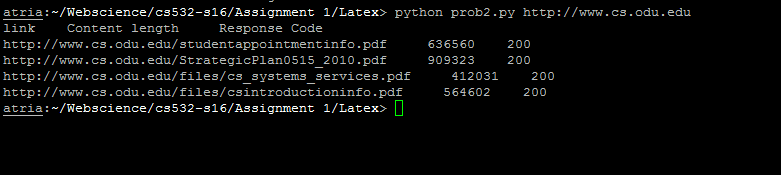
\includegraphics[scale=0.9]{sample_1.png}
        \caption{Output 1}
        \label{fig:X-distribution}
    \end{center}
\end{figure}
\newpage
\item To get the sample output 2 the following command should be executed 
\begin{verbatim}
python prob2.py http://www.cs.odu.edu/~mln/teaching/cs532-s16/test/pdfs.html
\end{verbatim}
\begin{figure}[ht]    
    \begin{center}
        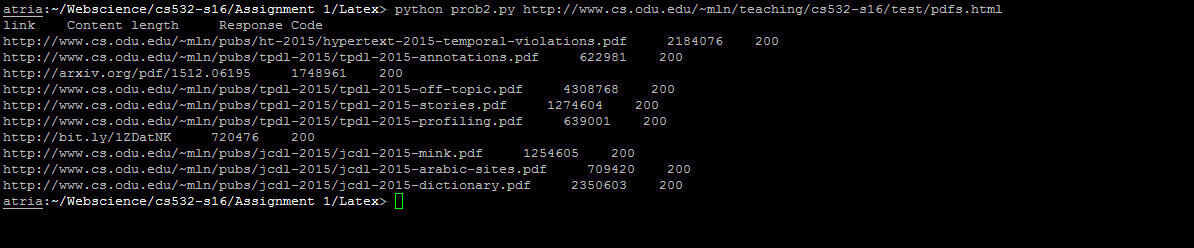
\includegraphics[scale=0.9]{sample_2.png}
        \caption{Output 2}
        \label{fig:X-distribution}
    \end{center}
\end{figure}
\item To get the sample output 3 the following command should be executed 
\begin{verbatim}
python prob2.py http://www.oracle.com/index.html
\end{verbatim}

\begin{figure}[ht]    
    \begin{center}
        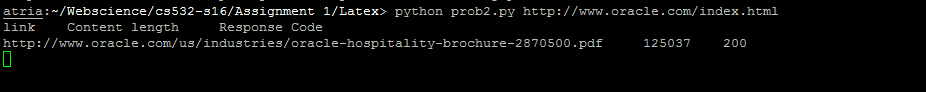
\includegraphics[scale=0.9]{sample_3.png}
        \caption{Output 3}
        \label{fig:X-distribution}
    \end{center}
\end{figure}
\end{enumerate}
\newpage
\subsection{Code Listing}
\lstinputlisting[language=Python, breaklines=true]{prob2.py}